\documentclass{article}
\usepackage{graphicx}
\usepackage{amssymb,amsmath}
\usepackage{subcaption} %That's for the subfigures
\usepackage{fullpage} %Use this if you have a problem with space.
\usepackage{tikz}
\usetikzlibrary{arrows}

\author{Stefano Duca \and Alexandros Rigos}
\title{Contracts in an Evolutionary Prisoner's Dilemma Game: A Report}

\begin{document}

\maketitle

\section{The main idea}
Here we are playing what we call a contract game in a prisoner's dilemma on a spatial lattice.

The idea is that a player can offer a part of what he earns ($\Delta$) to the other player to make it convenient to cooperate, conditional on the event of both players cooperating. Of course he might be tempted to defect but, due to the preference of errors, maybe the cooperation will be stable.

In its simplest form, the model we propose is the following:
\begin{itemize}
\item Agents are placed on a network, such as a ring, a Von Neumann lattice or a Moore lattice.

\item Agents play with their neighbours the following game:
\begin{center}
\begin{tabular}{|c|c|c|c|}
\hline 
$i 	\setminus j$ & C & D & $\Delta$ \\ 
\hline 
C & r,r & -a,1 & r+$\delta$, r-$\delta$ \\ 
\hline 
D & 1,-a & 0,0 & 1, -a \\ 
\hline 
$\Delta$ & r- $\delta$, r+$\delta$ & -a, 1 & r,r \\ 
\hline 
\end{tabular} 
\end{center}
The payoff matrix represents the game that we described above.
In addition to the cooperate and defect, an agent can choose to play the strategy $\Delta$ that represents the possibility of offering an unequal share of the cooperation reward to the other player.
The offer is a contract that states that in the case of the receiving player cooperating, it will receive an amount $\delta$ in addition to the cooperation reward.
The $\delta$ is taken from the share of the offering player so that there is no creation of wealth.
Hence $\delta \in \left[0,r \right]$.
In the case of two agents both offering the contract, each agent receives the fair cooperation payoff.
As usual in prisoner's dilemma games, $r$ indicates the reward and $a$ the sucker's payoff. Hence we have that $  -a < 0 < r < 1 $.

\item Agents can observe the payoffs obtained by their neighbours and imitate the strategy that seems to lead to the higher payoff.
We also allow for errors in the imitation function.
It is important to notice that due to the presence of errors it is possible for any strategy to emerge even if at a given time no agent on the network is playing it.
\end{itemize}


We implement the idea in several different ways:

\subsection{Logit best response:}
The players choose their strategy according to a logit best response with parameter beta, responding to the strategy array of the previous round.

This means that given an array of strategies $S^{t-1}$ at time $t-1$, player $i$ plays strategy $s_k$ at time $t$ with probability $p_k$ given by:
$$
p_{k}=\frac{e^{\beta EU\left(s_{k}\mid S_{-i}^{t-1}\right)}}{\sum_{s_{j}}e^{\beta EU\left(s_{j}\mid S_{-i}^{t-1}\right)}}
$$

where $ S_{-i}^{t-1}$ is the array representing the strategies of all agents but agent $i$
and $EU\left(s_{k}\mid S_{-i}^{t-1}\right)$ is the expected utility\footnote{Computed as the average payoff obtained by the interaction of $i$ with its nearest neighbours} of strategy $s_k$.

Below are some examples of results we obtained.
\begin{figure}[htbp] 
\centering
\begin{subfigure}[t]{0.47\textwidth}
  \centering
  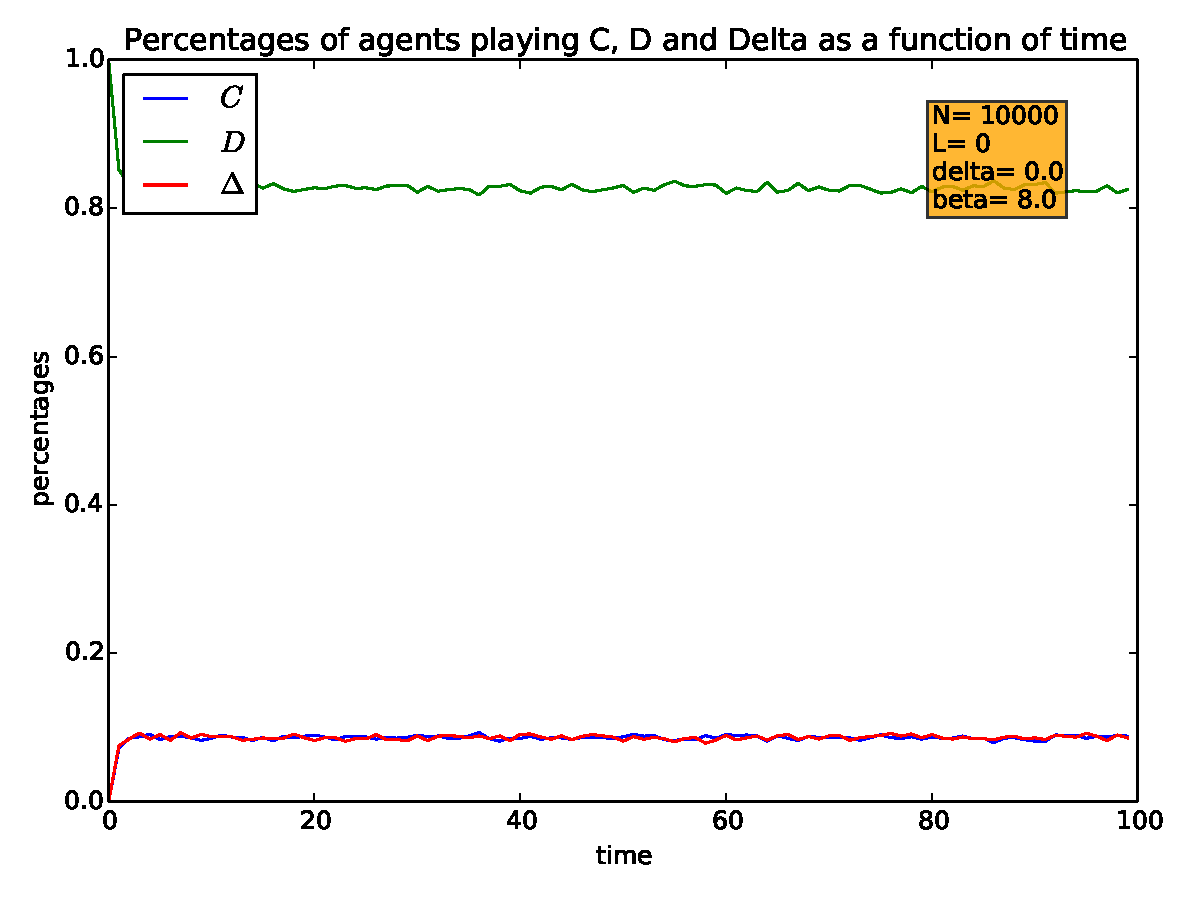
\includegraphics[width=\textwidth]{./Figures/BR_nodelta}
  \caption{Percentage of players playing each strategy in case the value of $\delta$ is 0.}
  \label{fig:BR_nodelta} 
\end{subfigure}%
~
~
\begin{subfigure}[t]{0.47\textwidth}
  \centering
  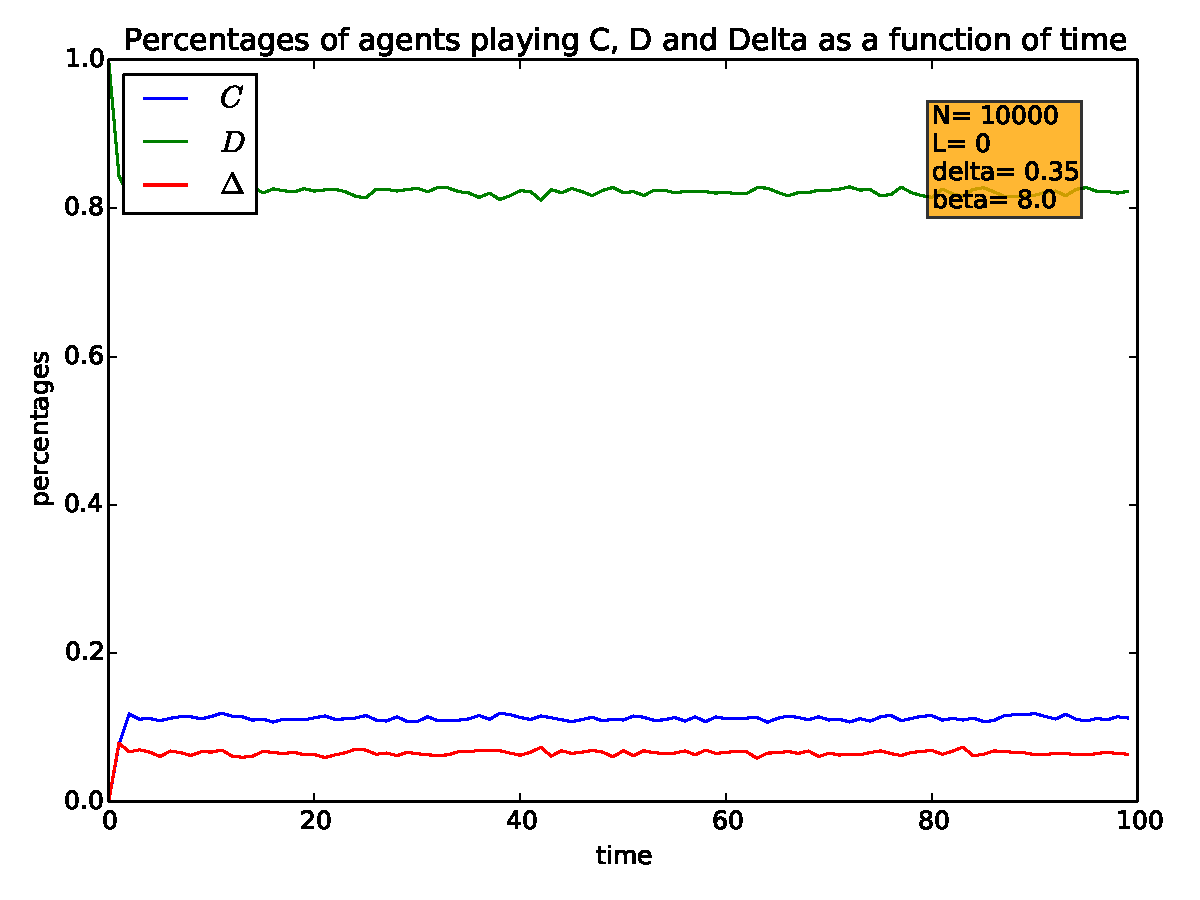
\includegraphics[width=\textwidth]{./Figures/BR_delta}
  \caption{Percentage of players playing each strategy in case the value of $\delta$ is $0.35$. Note that for this value $r+\delta >1$ and hence $C$ is the best response to $\Delta$.}
  \label{fig:BR_delta} 
\end{subfigure}
\caption{Percentage of players playing each strategy for two different values of $\delta$.
Fig (a) shows the percentage of players defecting (green line) in the case $\delta =0$. This is the case in which the strategy $\Delta$ is equivalent to cooperation.
We can see how in fig (b) there is no difference in the level of defection even though the value of $\delta$ is such that to cooperate is a best response to the strategy $\Delta$.
The kind of lattice used in the simulation is the Von Neumann lattice.
The picture is obtained in the case of agents choosing their strategy according to a logit best response.
}
\label{fig:BR}
\end{figure} 

Unfortunately, as shown in the picture, it seems that there is no difference in the level of cooperation between the "control case" where $\delta=0$ \ref{fig:BR_nodelta} and the case where $\delta>0$  \ref{fig:BR_nodelta} and such that to cooperate is a best response to $\Delta$.


\subsection{Logit best response with 4 strategies and directional transitions}
We now introduce another strategy: -Delta. Players that use this strategy, if their opponent cooperates, will take a larger part of the pie. More specifically, they will get $r+\Delta$ and their opponent will receive $r-\Delta$. The payoff matrix is, therefore amended to be the following:
\begin{center}
\begin{tabular}{|c|c|c|c|c|}
\hline 
• & C & D &+Delta & -Delta  \\ 
\hline 
C & $r$ , $r$ & $-a$ , 1 & $r+\Delta$, $r-\Delta$ & $r-\Delta$, $r+\Delta$ \\ 
\hline 
D & 1 , $-a$ & 0,0 & 1, $-a$ & 1,$-a$\\ 
\hline 
+Delta & $r -\Delta$, $r+\Delta$ & $-a$, 1 & $r$ , $r$& $r-2\Delta$, $r+2\Delta$ \\ 
\hline 
-Delta & $r+\Delta$ , $r-\Delta$ & $-a$, 1 & $r+2\Delta$ , $r-2\Delta$ & $r$ ,$ r$\\ 
\hline 
\end{tabular} 
\end{center}

Similarly as in previous cases, there is a logit rule in the way that agents switch stratetegies. Crucially, we allow only for specific transitions to tale place. These are shown in the following diagram. An arrow indicates a transition that is allowed. 

\begin{center}
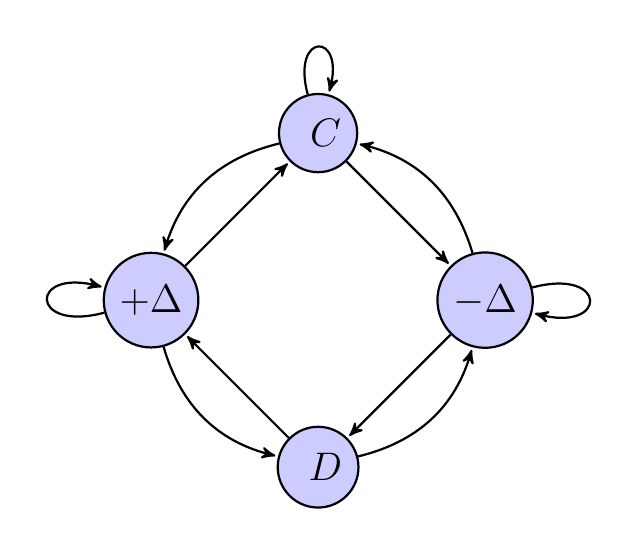
\begin{tikzpicture}[->,>=stealth',shorten >=1pt,auto,node distance=3cm,
  thick,main node/.style={circle,fill=blue!20,draw,font=\sffamily\Large\bfseries}]
  \node[main node] (1) {$~C$};
  \node[main node] (2) [below left of=1] {$+\Delta$};
  \node[main node] (3) [below right of=2] {$~D$};
  \node[main node] (4) [below right of=1] {$-\Delta$};

  \path[every node/.style={font=\sffamily\small}]
    (1) edge node [left] { } (4)
        edge [bend right] node[left] { } (2)
        edge [loop above] node { } (1)
    (2) edge node [right] { } (1)
	%edge node {} (4)
        edge [loop left] node {} (2)
        edge [bend right] node[left] {} (3)
    (3) edge node [right] {} (2)
        edge [bend right] node[right] {} (4)
    (4) edge node [left] {} (3)
        edge [loop right] node {} (4)
        edge [bend right] node[right] {} (1);
\end{tikzpicture}
\end{center}

Results show that the directional transitions do not change the percentage of cooperators in the long run (see the following figures).

Imitation

Imitation with delta conditional on last round's decisions.

\section{Future}

\subsection{Best responders with imitators}

\section{other ideas}
group scoring with stars and intermediate rounds of interaction
%\section{Notes on the code}
%\begin{enumerate}
%\item  So far we consider 3 types of lattice:
%0 stands for squared lattice with Von Neumann n.n. ;
%1 stands for squared lattice with Moore n.n.;
%2 stands for ring lattice.

%\item 0 is C, 1 is D and 2 is Delta
%\end{enumerate}

\end{document}
